\begin{title}
  Теория поверхностей
\end{title}

\begin{title}[\Large]
  Параграф 2.1
\end{title}

\begin{title}[\Large]
  Определение и примеры поверхностей в $R^3$. Локальное свойство регулярной
  поверхности
\end{title}

\begin{define}[непрерывной поверхности]
  Непрерывной поверхностью в $R^3$, называется
  непрерывное отображение $\varphi: U \subseteq R^2 \to R^3$, где
  $U$ открытое множество (множество, каждый элемент которого входит
  в него вместе с некоторой окрестностью)

  $(u, \upsilon) \in U ~~~ \vec \varphi(u, \upsilon) = (x(u, \upsilon),
  y(u, \upsilon), z(u, \upsilon))$

  $\vec \varphi (U) \subseteq R^2$ образ поверхности

  $\vec \varphi = (x(u, \upsilon), y(u, \upsilon), z(u, \upsilon))$ вектор
  функция
  $$
  \left\{
  \begin{array}{c}
    x = x(u, \upsilon) \\
    y = y(u, \upsilon) \\
    z = z(u, \upsilon)
  \end{array}
  \right. ~~~ \text{параметрическое уравнение поверхности}
  $$
  $\vec \varphi = \vec \varphi(u, \upsilon)$ называется гладкая если
  задающие ее координаты функции являются гладкими.
\end{define}

\begin{block}[Примеры]
  \begin{center}
    Top
  \end{center}
  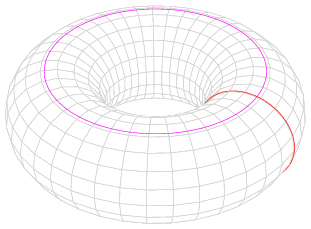
\includegraphics[width = 4.5cm]{Torus}
  $$
  \left\{
  \begin{array}{l}
    x = (a + b\cos u) \cos \upsilon \\
    y = (a + b\cos u) \sin \upsilon \\
    z = b \sin u
  \end{array}
  \right.
  $$
  \begin{center}
    Катеноид
  \end{center}
  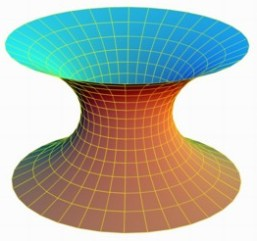
\includegraphics[width = 4.5cm]{katenoid}
  $$
  \left\{
  \begin{array}{l}
    x = a \ch \frac{u}{a} \cos \upsilon \\
    y = a \ch \frac{u}{a} \sin \upsilon \\
    z = u
  \end{array}
  \right.
  $$
  \begin{center}
    Псевдасфера
  \end{center}
  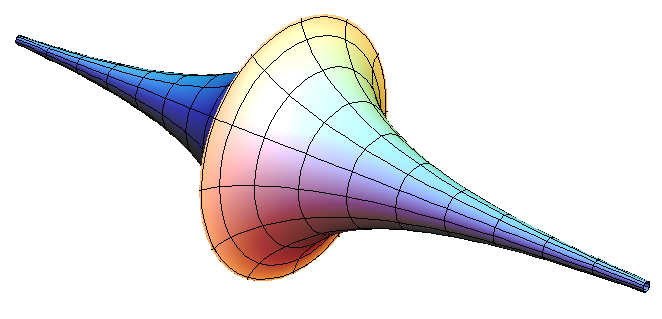
\includegraphics[width = 4.5cm]{pseudosphere}
  $$
  \left\{
  \begin{array}{l}
    x = a \sin u \cos \upsilon \\
    y = a \sin u \sin \upsilon \\
    z = a( \ln \tg \frac{u}{2} + \cos u)
  \end{array}
  \right.
  $$
\end{block}

\begin{define}
  Гладка поверхность $\vec \varphi = \vec \varphi
  (x(u, \upsilon), y(u, \upsilon), z(u, \upsilon))$ называется регулярной если
  $$
  \forall (u, \upsilon) ~~~
  \rang \left(
  \begin{array}{ccc}
    \frac{\partial x}{\partial u} & \frac{\partial y}{\partial u} &
    \frac{\partial z}{\partial u} \\
    \frac{\partial x}{\partial \upsilon} &
    \frac{\partial y}{\partial \upsilon} &
    \frac{\partial z}{\partial \upsilon}
  \end{array}
  \right) = 2 ~ \Leftrightarrow
  $$
  $\vec \varphi_u = (x_u, y_u, z_u) ~~~ \vec \varphi_{\upsilon} =
  (x_{\upsilon}, y_{\upsilon}, z_{\upsilon})$ линейно независимы
\end{define}

\begin{theorem}
  $\vec \varphi = \vec \varphi(u, \upsilon)$ гладкая поверхность и точка
  $(u_0, \upsilon_0) ~~ \vec \varphi_u (u_0, \upsilon_0),
  \vec \varphi_{\upsilon} (u_0, \upsilon_0)$ линейно независисмы, тогда
  $\exists (u, \upsilon) \in O(u_0, \upsilon_0) ~~ \varphi : (u, \upsilon)
  \to R^3$ инеъктивно
\end{theorem}

\begin{proof}
  Частный случай теоремы ниже
\end{proof}

\begin{block}[Следствие]
  Локально каждая точка образа поверхности однозначно определяется своими
  параметрами $(u, \upsilon)$ (невозможно что две точки проходят в одну точку
  образа)

  Будем говорит что $(u, \upsilon)$ задаются на поверхности локальную систему
  координат
\end{block}

\begin{theorem}
  $f: U \subseteq R^n \to R^m ~~ m \ge n$ гладкое отображение и точка
  $x_0 \in U ~~ \rang df(x_0) = n$ тогда $\exists x \in O(x_0) ~~
  f: x \to R^m$ инективно
\end{theorem}

\begin{proof}
  $f: U \subseteq R^2 \to R^3$

  $f = (x(u, \upsilon)), y(u, \upsilon), z(u, \upsilon))$ в каждой точке
  дифференциала это линейное отображение
  $$
  df =
  \left(
  \begin{array}{ccc}
    x_u & y_u & z_u \\
    x_{\upsilon} & y_{\upsilon} & z_{\upsilon} \\
  \end{array}
  \right)^T
  $$
  по условию $\rang df(u_0, \upsilon_0) = 2$ тогда по следствию из теоремы о
  неявной функции следует что $\exists (u, \upsilon) \in O(u_0, \upsilon_0) ~~
  f: (u, \upsilon) \to R^3$ инъективна
\end{proof}

\begin{title}[\Large]
  Теорема о регулярных поверхностях в пространстве, заданных неявным образом
\end{title}

\begin{theorem}
  $F(x,y,z)$ гладкая функция, $\exists (x_0, y_0, z_0) ~~ F(x_0, y_0, z_0) = 0$
  и
  $$
  \grad F(x_0, y_0, z_0) = \left(
  \frac{\partial F(x_0, y_0, z_0)}{\partial x},
  \frac{\partial F(x_0, y_0, z_0)}{\partial y},
  \frac{\partial F(x_0, y_0, z_0)}{\partial z}
  \right) \not= 0
  $$
  тогда $\exists x,y,z \in O(x_0, y_0, z_0) ~~ F(x, y, z) = 0$ является образом
  регулярной поверхности.

  В этом случае мы будем говорить что эта регулярная поверхность задана
  неявно уравнением $F(x, y, z) = 0$
\end{theorem}

\begin{proof}
  По условию в точке $(x_0, y_0, z_0)$
  $$
  \grad F(x_0, y_0, z_0) = \left( \frac{\partial F(x_0, y_0, z_0)}{\partial x},
  \frac{\partial F(x_0, y_0, z_0)}{\partial y}
  \frac{\partial F(x_0, y_0, z_0)}{\partial z} \right) \not= \vec 0
  $$
  $\frac{\partial F(x_0, y_0, z_0)}{\partial x} \not= 0$ или
  $\frac{\partial F(x_0, y_0, z_0)}{\partial y} \not= 0$ или
  $\frac{\partial F(x_0, y_0, z_0)}{\partial z} \not= 0$ $\Rightarrow$
  по теореме о неявной функции $\exists (x, y, z) \in O(x_0, y_0, z_0) ~~~
  F(x, y, z) = 0$ задается соотношением $z = f(x,y)$
  то есть состоит из точек вида $(x, y, f(x, y))$ $\Rightarrow$ это множество
  точек задается параметрически $(u, \upsilon, f(u, \upsilon))$
  $\Rightarrow$ $(1, \upsilon, f_u(u, \upsilon)) \not= \vec 0 ~~~
  (u, 1, f_{\upsilon}(u, \upsilon)) \not= \vec 0$ кривая
  заданная этим уравнением регулярная.
\end{proof}